\documentclass[12pt]{article}

%%%%%%%%%%%%%%%%%%%%%%%%%%%%%%%%%%%%%%%%%%%%%%%%%%%%%%%%%%%%%%%%%%%%%%%%
%% Customizações do abnTeX2 (http://abnTeX2.googlecode.com)           %%
%% para a Universidade Estadual do Ceara - UECE                       %%
%%                                                                    %%
%% This work may be distributed and/or modified under the             %%
%% conditions of the LaTeX Project Public License, either version 1.3 %%
%% of this license or (at your option) any later version.             %%
%% The latest version of this license is in                           %%
%%   http://www.latex-project.org/lppl.txt                            %%
%% and version 1.3 or later is part of all distributions of LaTeX     %%
%% version 2005/12/01 or later.                                       %%
%%                                                                    %%
%% This work has the LPPL maintenance status `maintained'.            %%
%%                                                                    %%
%% The Current Maintainer of this work is Thiago Nascimento           %%
%%                                                                    %%
%% Project available on: https://github.com/thiagodnf/uecetex2        %%
%%                                                                    %%
%% Further information about abnTeX2                                  %%
%% are available on http://abntex2.googlecode.com/                    %%
%%                                                                    %%
%%%%%%%%%%%%%%%%%%%%%%%%%%%%%%%%%%%%%%%%%%%%%%%%%%%%%%%%%%%%%%%%%%%%%%%%

% \documentclass[
%     a4paper,          % Tamanho da folha A4
%     12pt,             % Tamanho da fonte 12pt
%     chapter=TITLE,    % Todos os capitulos devem ter caixa alta
%     section=TITLE,    % Todas as secoes devem ter caixa alta
%     oneside,          % Usada para impressao em apenas uma face do papel
%     english,          % Hifenizacoes em ingles
%     spanish,          % Hifenizacoes em espanhol
%     brazil            % Ultimo idioma eh o idioma padrao do documento
% ]{abntex2}



% Importações de pacotes
\usepackage[utf8]{inputenc}                         % Acentuação direta
\usepackage[T1]{fontenc}                            % Codificação da fonte em 8 bits
\usepackage{graphicx}                               % Inserir figuras
\usepackage{amsfonts, amssymb, amsmath}             % Fonte e símbolos matemáticos
\usepackage{booktabs}                               % Comandos para tabelas
\usepackage{verbatim}                               % Texto é interpretado como escrito no documento
\usepackage{multirow, array}                        % Múltiplas linhas e colunas em tabelas
\usepackage{indentfirst}                            % Endenta o primeiro parágrafo de cada seção.
\usepackage{listings}                               % Utilizar codigo fonte no documento
\usepackage{xcolor}
\usepackage{microtype}                              % Para melhorias de justificação?
\usepackage[portuguese,ruled,lined]{algorithm2e}    % Escrever algoritmos
\usepackage{algorithmic}                            % Criar Algoritmos
\usepackage{float}                                  % Utilizado para criação de floats
\usepackage{amsgen}
\usepackage{lipsum}                                 % Usar a simulação de texto Lorem Ipsum
%\usepackage{titlesec}                               % Permite alterar os títulos do documento
\usepackage{tocloft}                                % Permite alterar a formatação do Sumário
\usepackage{etoolbox}                               % Usado para alterar a fonte da Section no Sumário
\usepackage[nogroupskip,nonumberlist,acronym]{glossaries}                % Permite fazer o glossario
\usepackage{caption}                                % Altera o comportamento da tag caption
\usepackage[num, abnt-emphasize=bf, bibjustif, recuo=0cm, abnt-etal-cite=2, abnt-etal-list=0]{abntex2cite}  % Citações padrão ABNT
%\usepackage[bottom]{footmisc}                      % Mantém as notas de rodapé sempre na mesma posição
%\usepackage{times}                                 % Usa a fonte Times
\usepackage{mathptmx}                               % Usa a fonte Times New Roman
%\usepackage{lmodern}                               % Usa a fonte Latin Modern
%\usepackage{subfig}                                % Posicionamento de figuras
%\usepackage{scalefnt}                              % Permite redimensionar tamanho da fonte
%\usepackage{color, colortbl}                        % Comandos de cores
%\usepackage{lscape}                                % Permite páginas em modo "paisagem"
%\usepackage{ae, aecompl}                           % Fontes de alta qualidade
%\usepackage{picinpar}                              % Dispor imagens em parágrafos
%\usepackage{latexsym}                              % Símbolos matemáticos
%\usepackage{upgreek}                               % Fonte letras gregas
\usepackage{appendix}                               % Gerar o apendice no final do documento
\usepackage{paracol}                                % Criar paragrafos sem identacao
\usepackage{lib/uecetex2}		                    % Biblioteca com as normas da UECE para trabalhos academicos
\usepackage{pdfpages}                               % Incluir pdf no documento
\usepackage{amsmath}                                % Usar equacoes matematicas

\usepackage{hyperref}

\usepackage{glossaries}

\usepackage{enumerate}
\usepackage{enumitem}

\renewcommand{\ABNTEXchapterfontsize}{\normalsize}

\renewcommand{\ABNTEXsectionfontsize}{\normalsize}

% Organiza e gera a lista de abreviaturas, simbolos e glossario
\makenoidxglossaries

% Gera o Indice do documento
\makeindex


\sloppy

\title{Uma Revisão de Literatura sobre \textit{Ferramentas Computacionais para o Estudo da Evolução de Espécies Baseado no Uso de Códons}}

\author{Mauricio Souza Menezes\\}
\address{Departamento de Ciências Exatas e da Terra, Campus I\\
Universidade do Estado da Bahia (UNEB)\\
Salvador, Bahia, Brasil.
  \email{mauriciosm95@gmail.com}
}

\begin{document}

\newacronym{ufm}{UFM}{Universal Feature Method}
\newacronym{ngs}{NGS}{Sequenciamento de Nova Geração}
\newacronym{ed}{ED}{Estruturas de Dados}
\newacronym{rs}{RS}{Revisão Sistemática}
\newacronym{cafe}{CAFe}{Comunidade Acadêmica Federada}

\maketitle

\begin{resumo}
    Aqui deve ser colocado o resumo do relatório da revisão sistemática, descrevendo os pontos mais importantes, como os objetivos da revisão, principais questões-problema, e principais resultados obtidos.
\end{resumo}


\begin{abstract}
    \begin{otherlanguage}{english}
        You should put here the abstract summarizing your sistematic review report. You are supposed to describe the main points in your report: review goals, main research questions and main results achieved.
    \end{otherlanguage} \textcolor{red}{Atenção ! Não faça tradução automática do resumo usando o Google ou outro tradutor automático. Se fizer isto, o Abstract ficará de péssima qualidade. Reescreva o Resumo em inglês e não apenas o traduza. A ideia expressada é que deve se a mesma e não as palavras.}
\end{abstract}


\section{Introdução}

Este artigo apresenta uma \gls{rs} da literatura referente a utilização do método \gls{ufm} no processamento da saída dos equipamentos \gls{ngs} em vírus de alta relevância epidemiológica. A artigos foram obtidos através da busca realizada em sete bases de dados(ACM, BioRxiv, Elsevier, Google Scholar, IEEE, PubMed, e Spring) levando em conta a principal questão: Se o método \gls{ufm}, pode ser utilizado para processar os fragmentos de DNA/RNA viral, obtidos com as técnicas de \gls{ngs}? Foram incluídos todos os artigos que atenderam os critérios definidos.
Nos cursos da área de computação, a disciplina de \gls{ed} serve como base para a maioria das matérias posteriores, apesar disso, ainda existe grande dificuldade relacionada ao seu ensino. Sendo assim, várias metodologias foram propostas ao longo do tempo, e uma dessas propostas foi o ensino de \gls{ed} com a utilização de jogos.

\section{Relato da Revisão de Literatura}

Logo após identificar o problema de dificuldades no ensino de \gls{ed}, foi necessário conhecer os pormenores que estavam relacionados a mesma. Para isso, foi necessário realizar uma \gls{rs}. Foi utilizado um protocolo, que serviria como base no processo para a obtenção dos estudos que deveriam ser analisdos. As definições feitas no protocolo foram as seguintes: Questões de pesquisa, palavras-chave, critérios de busca, fontes de pesquisa, críterios para inclusão e exclusão e string de busca.

As palavras-chave utilizadas foras as seguintes: Aprendizagem; Metodologia de ensino; Estruturas de dados; jogo; Hora do rush.
Elas foram definidas com o objetivo de encontrar o máximo de estudos relevantes que pudessem responder as questões de pesquisa. É importante salientar que foram também utilizadas as respectivas palavras em Inglês e Espanhol, pois também foram considerados estudos nesses idiomas.

\subsection{Objetivo da Pesquisa}

A pesquisa teve como objetivo a obtenção do conhecimento fundamental sobre a área, a identificação do que já foi feito para sanar o problema identificado e também se era viável ou não o desenvolvimento de uma solução nova para o ensino de \gls{ed} com jogos.

\subsection{Questões de Pesquisa}

Foram definidas três questões de pesquisa. A primeira e principal foi: "Quais metodologias são utilizadas para ensinar estruturas de dados com jogos?", já as duas questões secundárias foram: "Quais jogos são utilizados para ensinar estruturas de dados?" e "O jogo Hora do Rush já foi utilizado, de alguma forma, para ensinar estruturas de dados?".

As questões de pesquisa foram escolhidas com base naquilo que se queria entender ao final da \gls{rs}.

\subsection{Repositório de Busca de Dados}

Para a obtenção dos estudos foram utilizados as seguintes bases de dados:
\begin{itemize}
    \item{ACM Digital Library}
    \item{\gls{ceie}}
    \item{\gls{ieee}}
    \item{\gls{scielo}}
    \item{Springer}
\end{itemize}

As bases foram escolhidas principalmente por conta da conceituação dos trabalhos que possuem. Um dos críterios utilizados para tal escolha foi o sistema Qualis Capes. Também foi possível, através dessas bases, a obtenção dos estudos de forma completa e na sua maioria de forma gratuita, sendo importante salientar, que para que isso fosse possível, foi necessário realizar o acesso remoto por meio do portal da \gls{cafe} que é um serviço provido pela \gls{rnp}.

\subsection{Palavras-chave e Strings de Busca}

As palavras-chave selecionadas para a busca nas bases de dados, com o objetivo de encontrar o máximo de estudos relevantes, foram as seguintes:
\begin{itemize}
    \item{Aprendizagem}
    \item{Dificuldade de aprendizagem}
    \item{Estruturas de dados}
    \item{Hora do rush}
    \item{Jogo}
    \item{Metodologia de ensino}
    \item{Objeto de aprendizagem}
\end{itemize}

A tabela a seguir apresenta as strings de busca utilizadas em suas respectivas bases de dados. É importante salientar, que a depender da base de dados, também foram utilizados os correlatos em espanhol e inglês das palavras-chave, para que o máximo de trabalhos relevantes fossem encontrados.

\begin{table}[h]
    \centering

    \caption{STRINGS DE BUSCA NAS BASES DE DADOS}
    \label{fig:stringBuscaBase}
    \begin{tabular}{|p{2cm}|p{10cm}|}
        \hline
        BASE DE DADOS        & STRING BUSCA                                                                                                                                                                                                                                       \\
        \hline
        STRING GERAL         & ("Estruturas de Dados" OR "Data Structures") AND (("Learning" OR "Aprendizagem") OR ("Metodologia de Ensino" OR "Teaching Methodology")) AND (("Jogo" OR "Game") OR ("Hora do Rush" OR "Rush Hour"))                                               \\
        \hline
        ACM Digital Library  & "Data Structures" AND ("Learning Object" OR "Teaching Methodology" OR "Learning Difficulty" OR "Learning Teaching") AND ("Game" OR "Rush Hour")                                                                                                    \\
        \hline
        CEIE                 & "Data Structure" OR "Estruturas de Dados"                                                                                                                                                                                                          \\
        \hline
        IEEE Digital Library & ("Estruturas de Dados" OR "Data Structures") AND (("Learning" OR "Aprendizagem") OR ("Metodologia de Ensino" OR "Teaching Methodology")) AND (("Jogo" OR "Game") OR ("Hora do Rush" OR "Rush Hour"))                                               \\
        \hline
        SciELO               & ("Estruturas de Dados" OR "Data Structure" OR "Estructuras de datos") AND ("Aprendizagem" OR "Learning" OR "Aprendiendo" OR "Ensino" OR "Enseñando" OR "Teaching" OR "Jogo" OR "Games" OR "Juego" OR "Hora do Rush" OR "Rush Hour" OR "Hora Pico") \\
        \hline
        Springer             & "Data Structures" AND ("Learning Object" OR "Teaching Methodology" OR "Learning Difficulty" OR "Learning Teaching") AND ("Game" OR "Rush Hour")                                                                                                    \\
        \hline
    \end{tabular}

\end{table}

\subsection{Critérios de busca}

Para realizar o processo de seleção dos estudos foram definidos críterios, podendo ser de inclusão ou de exclusão.

Os critérios de inclusão foram os seguintes:
\begin{itemize}
    \item O estudo aborda o ensino de \gls{ed}.
    \item O estudo aborda o uso de jogos para o ensino de \gls{ed}.
    \item O estudo contém as palavras-chave definidas na pesquisa no resumo, titulo ou palavras-chave.
    \item O estudo possui o texto completo disponível.
\end{itemize}
Os critérios de exclusão foram os seguintes:
\begin{itemize}
    \item O resumo não define claramente o objetido do estudo.
    \item O estudo está duplicado.
    \item É necessário o pagamento de uma taxa para acesso ao estudo.
    \item O estudo não está escrito em português, inglês ou espanhol.
    \item O tema do estudo não está relacionado ao ensino de \gls{ed}.
\end{itemize}

\section{Resultados Parciais}

Nesta subseção devem ser apresentados os resultados parciais após a etapa de seleção dos trabalhos. Indicando a quantidade total de artigos retornados pela busca nas bases, a quantidade de arquivos selecionados, indicando a distribuição por critérios de inclusão/exclusão. Enfim, uma análise quantitativa dos trabalhos e qualitativa indicando se as principais questões de pesquisa tendem a ser respondidas, considerando os critérios de inclusão mapeados.

Observem que esta etapa de seleção prevê a leitura apenas do título, abstract e palavras-chave dos artigos. Desta forma faz-se a seleção inicial do que será de fato lido a fundo.

Para retratar estes dados, podem ser usados gráficos e figuras formatados como no exemplo da Figura \ref{fig:depth}. Se usar a ferramenta STArt, pode incluir no relatório alguns gráficos e tabelas gerados pela ferramenta que refletem bem esta etapa da revisão sistemática.

\subsection{Análise Qualitativa dos Resultados}

Esta subseção reflete o resultado da extração de dados. Depois de extrair as informações úteis através da leitura completa dos artigos selecionados, o autor deve descrever aqui sua análise qualitativa do que encontrou durante a pesquisa, citando os principais artigos e as informações relevantes que encontrou para responder às questões de pesquisa definidas no protocolo da revisão sistemática. Também podem ser usadas figuras e tabelas para fundamentar a análise.

Observe que alguns artigos que foram originalmente selecionados para leitura, podem ser excluídos por algum dos critérios de exclusão definido após a leitura completa. Neste caso a planilha-resumo deve ser atualizada.

\begin{figure}[tb]
    \centering
    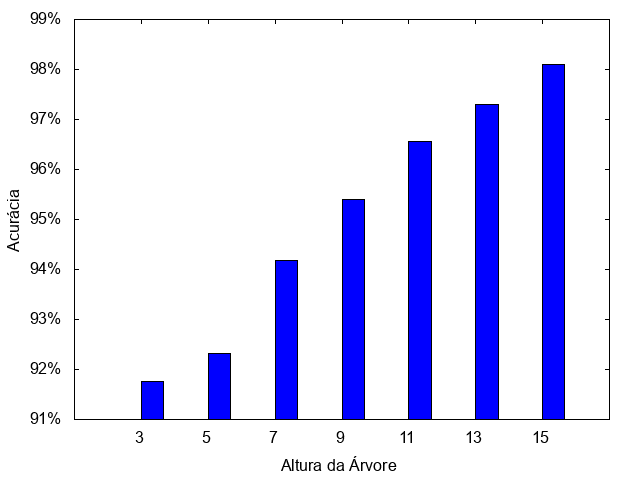
\includegraphics[scale=0.7]{tree-depth.png}
    \caption{Exemplo genérico de um gráfico ou figura que pode ser colocao aqui para representar os resultados quantitativos.}
    \label{fig:depth}
\end{figure}

\section{Conclusões}

Aqui o autor deve fazer uma reflexão sobre os achados da revisão sistemática. Esteja atento para acrescentar informação nova, ou seja, para "Concluir" de fato alguma coisa e não para repetir a análise da seção anterior.

Devem ser inclusive apontadas as lacunas e limitações identificadas a partir da revisão sistemática, fazendo link com as possíveis propostas que serão apresentadas futuramente no anteprojeto. Ou seja, a conclusão deste relatório deve preparar o alicerce para a construção do anteprojeto de pesquisa.



\bibliographystyle{sbc}
\bibliography{RefDoc}

\pagebreak
\begin{landscape}


    \section{Planilha-resumo de Resultados}

    Aqui deve ser atualizada a planilha-resumo contendo todos os trabalhos selecionados após a fase de seleção. A tabela deve conter todas as colunas indicadas a seguir com as informações relevantes sobre os trabalhos lidos na íntegra. Ver o exemplo na Tabela \ref{tab:resumo}.

    \begin{center}


        \begin{longtable}{p{8cm}|c|c|c|c|c|p{7cm}|p{5cm}}
            \caption{Planilha-resumo dos trabalhos selecionados.}
            \label{tab:resumo}                                                                                                                                                                                                                                                                                                                                                            \\
            \multicolumn{1}{c|}{\textbf{Identificação do Trabalho}} &
            \multicolumn{1}{c|}{\textbf{I1}}                        &
            \multicolumn{1}{c|}{\textbf{I2}}                        &
            \multicolumn{1}{c|}{\textbf{I3}}                        &
            \multicolumn{1}{c|}{\textbf{E1}}                        &
            \multicolumn{1}{c|}{\textbf{E2}}                        &
            \multicolumn{1}{c|}{\textbf{Descrição}}                 & \multicolumn{1}{c}{\textbf{Avaliação}}                                                                                                                                                                                                                                                                              \\ \hline \hline
            \endfirsthead

            \multicolumn{8}{c}%
            {{\bfseries \tablename\ \thetable{} -- continuação da página anterior}}                                                                                                                                                                                                                                                                                                       \\
            \multicolumn{1}{c|}{\textbf{Identificação do Trabalho}} &
            \multicolumn{1}{c|}{\textbf{I1}}                        &
            \multicolumn{1}{c|}{\textbf{I2}}                        &
            \multicolumn{1}{c|}{\textbf{I3}}                        &
            \multicolumn{1}{c|}{\textbf{E1}}                        &
            \multicolumn{1}{c|}{\textbf{E2}}                        &
            \multicolumn{1}{c|}{\textbf{Descrição}}                 & \multicolumn{1}{c}{\textbf{Avaliação}}                                                                                                                                                                                                                                                                              \\ \hline \hline
            \endhead

            \hline \multicolumn{8}{r}{{Continua na próxima página}}                                                                                                                                                                                                                                                                                                                       \\
            \endfoot
            \hline \hline
            \endlastfoot


            \bibentry{Laranjeira2015}                               & X                                      &   &   &  &   & Aqui é colocada a descrição do artigo com os dados resultantes da etapa de extração, após leitura completa do trabalho. & Aqui é feita avaliação do que foi encontrado neste artigo. Esta informação será útil para a avaliação qualitativa dos resultados. \\
            \hline
            \bibentry{breiman2017classification}                    &                                        &   & X &  & X & Aqui é colocada a descrição do artigo com os dados resultantes da etapa de extração, após leitura completa do trabalho. & Aqui é feita avaliação do que foi encontrado neste artigo. Esta informação será útil para a avaliação qualitativa dos resultados. \\
            \hline
            \bibentry{SimoesEtAl2016-BRAHUR}                        &                                        & X & X &  &   & Aqui é colocada a descrição do artigo com os dados resultantes da etapa de extração, após leitura completa do trabalho. & Aqui é feita avaliação do que foi encontrado neste artigo. Esta informação será útil para a avaliação qualitativa dos resultados. \\
            \hline
        \end{longtable}


    \end{center}

\end{landscape}
\end{document}
